\documentclass[xcolor=dvipsnames]{beamer}
\usepackage{subfig}
\usepackage{wrapfig}
\usetheme{Rochester}  %% Themenwahl
\usecolortheme[named=RoyalBlue]{structure}
\usebackgroundtemplate{
	\centering
	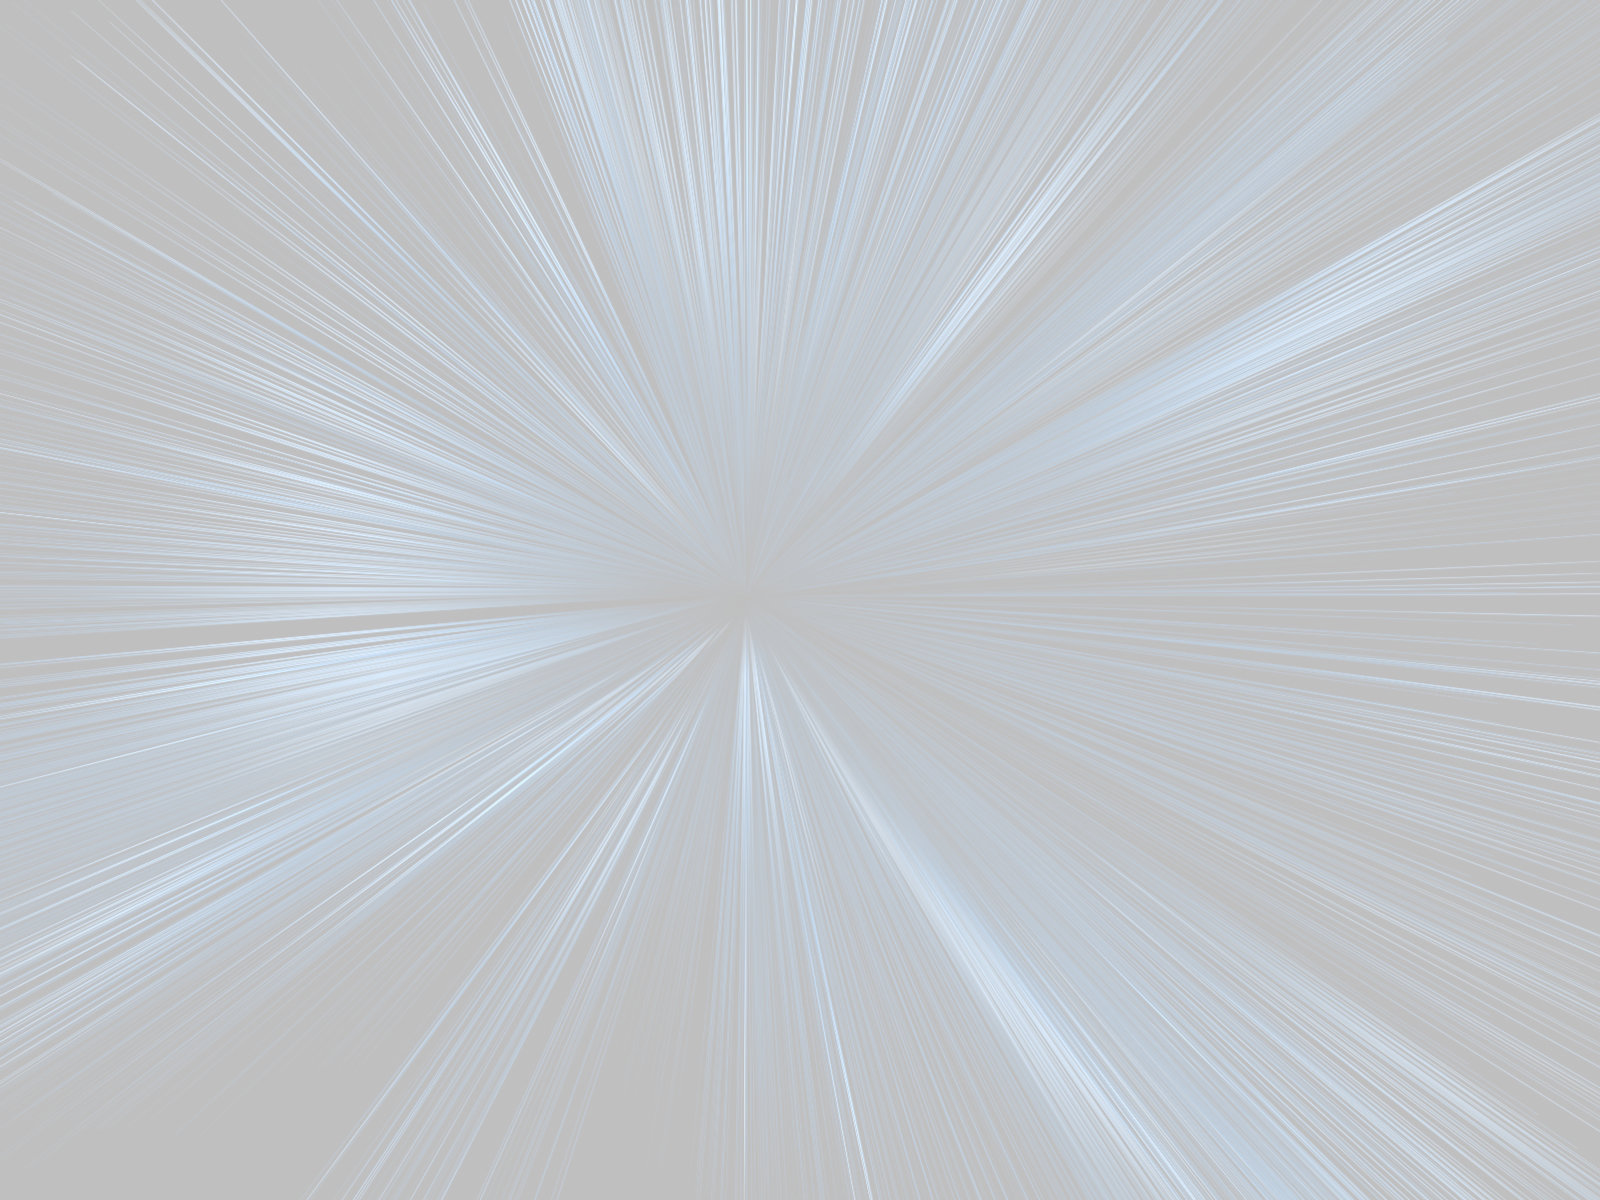
\includegraphics[width=\paperwidth,height=\paperheight]{images/light-speed}
} 

 \addtobeamertemplate{block begin}{\pgfsetfillopacity{0.5}}{\pgfsetfillopacity{1}}
 \addtobeamertemplate{block alerted begin}{\pgfsetfillopacity{0.5}}{\pgfsetfillopacity{1}}
 \addtobeamertemplate{block example begin}{\pgfsetfillopacity{0.5}}{\pgfsetfillopacity{1}}

\setbeamertemplate{navigation symbols}{}

\title{Solve'n Slide}
\subtitle{Interim Presentation}
\author{Hanieh Arjomand-Fard\\Kevin Sawischa\\Markus Ansorge\\Stefan Aicher}
\date{02. June 2017}

\begin{document}
	\maketitle
	
	\begin{frame}
		\frametitle{Basic Character and UI}
		\begin{itemize}
			\item Basic character implementation
			\begin{itemize}
				\item Handling of keyboard inputs
				\item Responsible for phase switch
				\item Connect different scripts via well defined interfaces
			\end{itemize}
			\item User interface
			\begin{itemize}
				\item Currently text only
				\item Will be replaced with (animated) textures in next milestone
			\end{itemize}
			\item Input scheme
			\begin{itemize}
				\item WASD+Space for movement, mouse to look around
				\item Left MB to raise, right MB to lower terrain
				\item Enter to switch phases, restart after death and go to next level
			\end{itemize}
		\end{itemize}
	\end{frame}
	
	\begin{frame}
		\frametitle{Terrain Manipulation}
		\begin{itemize}
			\item Player can manipulate terrain through mouse clicks
			\item Still needs balancing of intensity
			\item Redo option still needs to be implemented
			\item Caution: Unity stores terrain changes permanently
		\end{itemize}
			\begin{figure}[ht]
				\begin{tabular}{cc}
					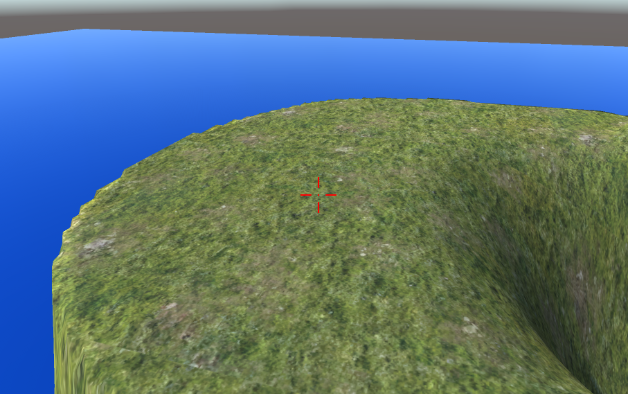
\includegraphics[scale=0.3]{images/interim/terrainManipulation1}&
					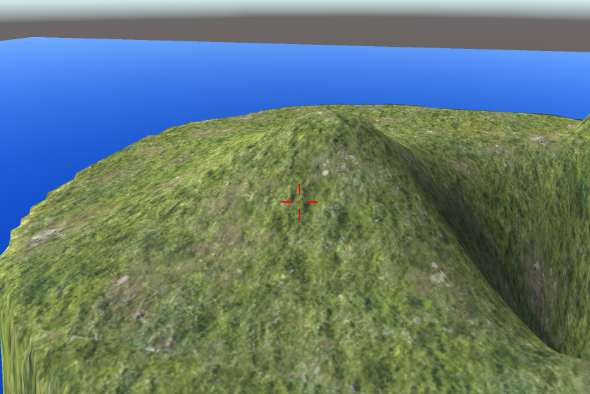
\includegraphics[scale=0.3]{images/interim/terrainManipulation2}
				\end{tabular}
			\end{figure}
	\end{frame}
	
	\begin{frame}
		\frametitle{Terrain River}
		\begin{itemize}
			\item Simulation based on heightmap
			\item Two repeating steps:
			\begin{itemize}
				\item River: path along lowest neighbor
				\item Lake: fill sink
			\end{itemize}
		\end{itemize}
		\begin{figure}[ht]
			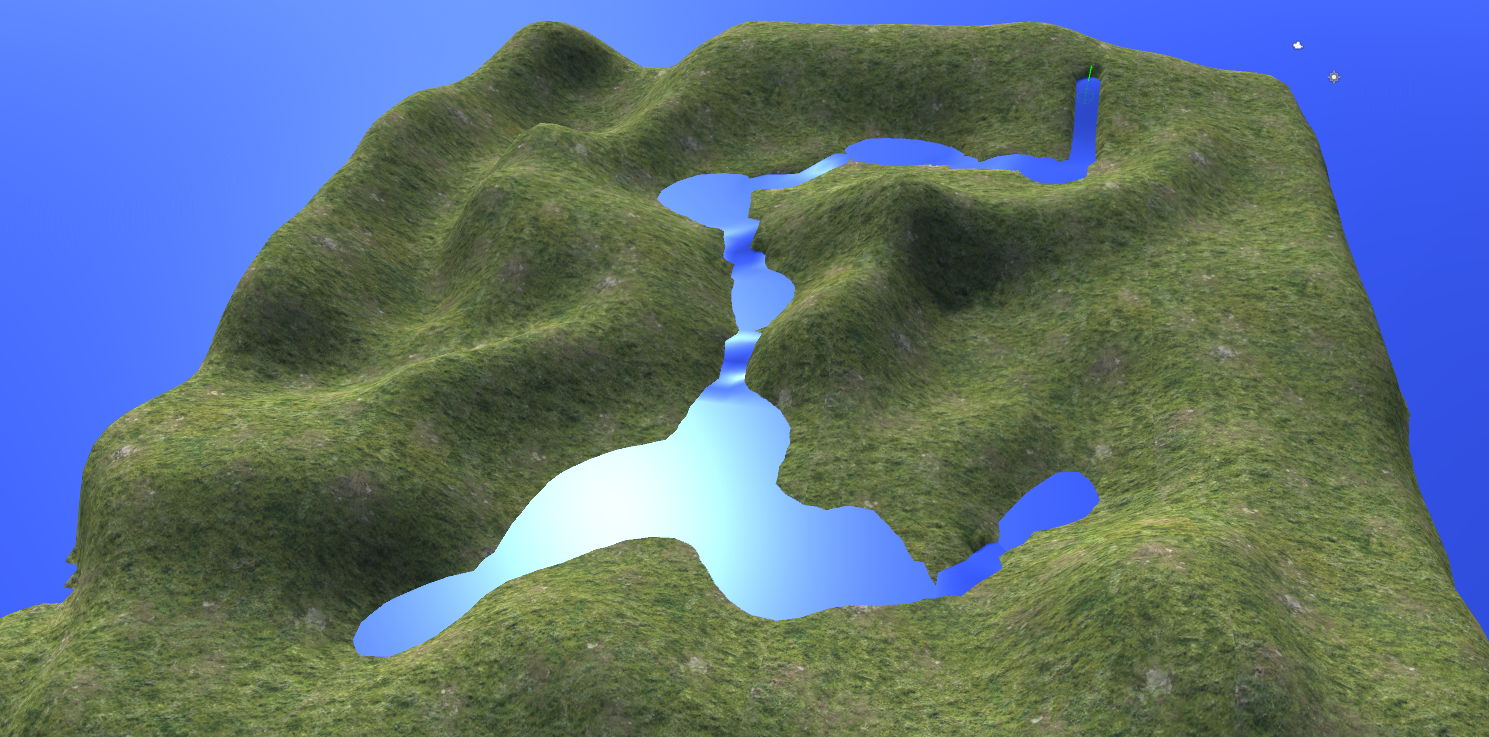
\includegraphics[scale=0.21]{images/interim/river1}
		\end{figure}
		\begin{itemize}
			\item Original plan: include velocity
		\end{itemize}
	\end{frame}
	
	\begin{frame}
		\frametitle{Modeling and Arts}
		\begin{columns}[T]
			\begin{column}{0.7\textwidth}
				\begin{itemize}
					\item Modeling with Blender
					\item Turret coding and animation in Unity
					\begin{itemize}
						\item Turrets aiming at the character
					\end{itemize}
					\item Character animation with Blender
				\end{itemize}
				\begin{figure}[ht]
					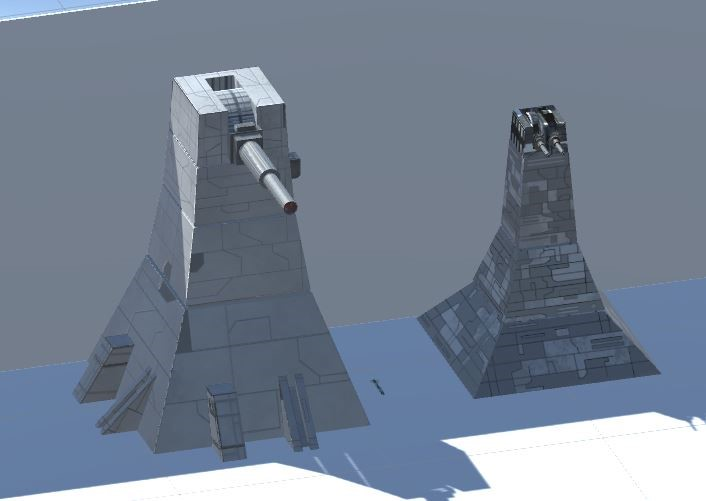
\includegraphics[scale=0.35]{images/interim/turrets}
				\end{figure}
			\end{column}
			\begin{column}{0.3\textwidth}
				\begin{figure}[ht]
					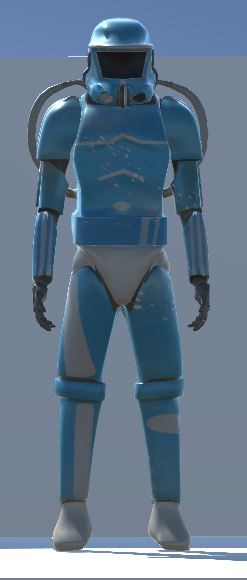
\includegraphics[scale=0.455]{images/interim/character}
				\end{figure}
			\end{column}
		\end{columns}
	\end{frame}
	
	\begin{frame}
		\frametitle{Demo}
		\centering
		\Huge
		Time for a live demo!
	\end{frame}
\end{document}